\documentclass[11pt,a4paper]{report}
%%%%%%%%%%%%%%%%%%%%%%%%%%%%%%%%%%%%%%%%%%%%%%%%%%%%%%%%%%%%%%%%%%%%%
%%                                                                 %%
%%    Header file for the Phi-S-X Series                           %%
%%                                                                 %%
%%    german version header_gm.tex is derived from header.tex      %%
%%    by uncommenting the line ``\setboolean{german}{true}'' below %%
%%                                                                 %%
%%    Never edit the german version! all changes must be done      %%
%%    in the english version header.tex                            %%
%%                                                                 %%
%%%%%%%%%%%%%%%%%%%%%%%%%%%%%%%%%%%%%%%%%%%%%%%%%%%%%%%%%%%%%%%%%%%%%
%%%%%%%%%%%%%%%%%%%%%%%%%%%%%%%%%%%%%%%%%%%%%%%%%%%%%%%%%%%%%%%%%%%%%
%%                                                                 %%
%%    Header file for the Phi-S-X Series                           %%
%%                                                                 %%
%%    german version header_gm.tex is derived from header.tex      %%
%%    by uncommenting the line ``\setboolean{german}{true}'' below %%
%%                                                                 %%
%%    Never edit the german version! all changes must be done      %%
%%    in the english version header.tex                            %%
%%                                                                 %%
%%%%%%%%%%%%%%%%%%%%%%%%%%%%%%%%%%%%%%%%%%%%%%%%%%%%%%%%%%%%%%%%%%%%%
%====================================================================
%-- define flag for language adaptations
\usepackage{ifthen}   % allows to select only certain text
\provideboolean{german}
\setboolean{german}{false}
%\setboolean{german}{true}  % uncomment this line for german editions
%====================================================================
%
% Textschriftart: Computer modern Bright
% body:            CM-Bright 10pt
% section titles:  CM-Bright Bold
% formulas:        CM-Bright Math Oblique
%
\usepackage[standard-baselineskips]{cmbright}
\usepackage{cmbright}
\usepackage[T1]{fontenc}
\def\usedfonts{CM-Bright}
\usepackage{typearea}
%\typearea[current]{calc} % benutzt die aktuelle 
       % bindekorrektur (BCOR angabe als parameter in koma usepackage)
       % und berechnet satzspiegel neu
\typearea[current]{11} %fixed div value

\usepackage{textcomp} % special symbols
\usepackage{amsfonts} % special symols
                      % see ftp://ftp.ams.org/pub/tex/doc/amsfonts/amsfndoc.pdf
\usepackage{amssymb}  % CM-Bright provides the AMS symbols
\usepackage{exscale}  % allows to scale math expressions to big fonts, 
                      % e.g. \Huge
\usepackage{curves}
\usepackage{braket}
\usepackage{miller}     % miller indices
\usepackage{chemmacros} % http://www.mychemistry.eu/mychemistry/
\usepackage[numbers]{natbib}     % bibliography style
\usepackage{url}\urlstyle{tt}
\usepackage{float}
\usepackage{bm}       % provides the command \bm{} that makes bold math symbols
\usepackage{amsmath}
\usepackage{amsbsy}   % allows bold mathematical symbols
\usepackage{amscd}
 \usepackage{a4wide}  % it is better to use the ``geometry'' package
\usepackage{array}    % 
\usepackage{fancyhdr} %  defines pagestyle fancy
\usepackage{epsfig}   % include graphics with epsfig
\usepackage{graphicx} % includegraphics
\usepackage{epstopdf}
\usepackage{wrapfig}
\usepackage{fancybox} % allows shadow-boxes
\usepackage{color}    % allows to use color in the text
%\usepackage{eepic}
\usepackage{flafter}  % places picture next to its reference
\usepackage{makeidx}  % make an index
%\usepackage{MnSymbol}  % 
%\usepackage{marvosym}  % 
\usepackage{textcase}
\usepackage{ulem} % defines strikeout \sout{}; underline \uline{}
                  % double underline \uuline{}; wave underline \uwave{}
                  % cross out \xout{}
%
%==========================================================================
%==  page layout  =========================================================
%==========================================================================
% eqnarray environment: reduce with of space in place of each ``&''
\setlength\arraycolsep{1.4pt}
\pagestyle{fancy}
%\renewcommand{\chaptermark}[1]{\markboth{\thechapter\ #1}{}}
\renewcommand{\chaptermark}[1]{\markboth{\MakeUppercase{\thechapter\ #1}}{}}
\fancyhf{} 
\fancyhead[LE]{\textsc{\thepage}\qquad\textsc{\leftmark}}
\fancyhead[RO]{\textsc{\leftmark}\qquad\textsc{\thepage}}
\renewcommand{\headrulewidth}{0.5pt}
\renewcommand{\footrulewidth}{0pt} 
\addtolength{\headheight}{2.5pt}
\fancypagestyle{plain}{\fancyhead{}
   \renewcommand{\headrulewidth}{0pt}
   \fancyfoot[CO]{\bfseries\thepage}}

% Line spacing -----------------------------------------------------------
\newlength{\defbaselineskip}
\setlength{\defbaselineskip}{\baselineskip}
\newcommand{\setlinespacing}[1]%
           {\setlength{\baselineskip}{#1 \defbaselineskip}}
\newcommand{\doublespacing}{\setlength{\baselineskip}%
                           {2.0 \defbaselineskip}}
\newcommand{\singlespacing}{\setlength{\baselineskip}{\defbaselineskip}}

% Absatz einr\"ucken ------------------------------------------------------
%\setlength{\parindent}{0pt}
\setlength{\parskip}{2pt}
% -------------------------------------------------------------------------
\ifthenelse{\boolean{german}}
  {\def\figurename{Abb.}}
  {\def\figurename{Fig.}}
%--------------------------------------------------------------------------
\renewcommand{\arraystretch}{1.15}  % skaliert den Zeilen abstand in der 
    % tabular und array umgebung
%
%==========================================================================
%==  boxes etc ============================================================
%==========================================================================
%== minipage in a shadowbox ===============================================
\newenvironment{myshadowminipage}[1]%
  {\par\noindent\begin{Sbox}\begin{minipage}{\linewidth}\vspace{0.1cm}\begin{center}\uppercase{#1}\end{center}}%
  {\vspace{0.1cm}\end{minipage}\end{Sbox}\shadowbox{\TheSbox}}
%
%== minipage in a framedbox ===============================================
\newenvironment{myframedminipage}%
  {\par\noindent\begin{Sbox}\begin{minipage}\linewidth\vspace{0.1cm}}%
  {\vspace{0.1cm}\end{minipage}\end{Sbox}\fbox{\TheSbox}}
%
\newcommand{\myshadowbox}[1]{\noindent\shadowbox{\parbox{\linewidth}{\smallskip #1\smallskip}}}
\newcommand{\myfbox}[1]{\noindent\fbox{\parbox{\linewidth}{\smallskip #1\smallskip}}\medskip}
%== minipage in a framedbox ===============================================
\newtheorem{defi}{Definition}[chapter]
\newenvironment{definition}[1]%
  {\par\noindent\begin{Sbox}\begin{minipage}{\linewidth}\vspace{0.1cm}\begin{defi}\uppercase{#1}\\\vspace{0.1cm}}%
  {\vspace{0.1cm}\end{defi}\end{minipage}\end{Sbox}\shadowbox{\TheSbox}}
%
%=========================================================================
% color used to point out information to the teacher
\definecolor{highlight}{rgb}{1.0,0.7,0.}
\newcommand{\Special}[1]{\textbf{\textcolor{highlight}{#1}}}
%=========================================================================
%  switch certain parts on and off. uses ifthen package
\newboolean{teacher}\setboolean{teacher}{false}
% this parameter can be changed in the manuscript again
\setboolean{teacher}{true} %private version if true!
\newcommand{\teacheronly}[1]{\ifthenelse{\boolean{teacher}}{#1\hfill\\ }}
\newcommand{\editor}[1]{\textcolor{blue}{\texttt{Editor: #1}}}
\newcommand{\MARK}[1]{\textcolor{blue}{#1}} 
\newcommand{\RED}[1]{\textcolor{red}{#1}} 
%
%==========================================================================
%==  define new symbols                                                 ===
%==========================================================================
% define \stat (stationary state) as an operator like \min
\DeclareMathOperator*{\stat}{stat}
\let\Vec=\mathbold   % cmbright.sty provides a bold/italic math alphabet
\let\Dot=\mathbold   % cmbright.sty provides a bold/italic math alphabet
\let\Ddot=\mathbold   % cmbright.sty provides a bold/italic math alphabet
%
\newcommand{\e}[1]{\mathrm{e}^{#1}}% exponential function
\renewcommand{\Re}{\mathrm{Re}}    % real part
\renewcommand{\Im}{\mathrm{Im}}    % imaginary part
\newcommand{\lagr}{\ell}           % Lagrange dichte
\newcommand{\Lagr}{\mathcal{L}}    % Lagrange Funktion
\newcommand{\erf}{{\rm erf}}       %
\newcommand{\atan}{{\rm atan}}     % arcus tangens
\newcommand{\mat}[1]{\bm{#1}}  % Matrix
\newcommand{\gmat}[1]{{\boldsymbol #1}}  % Matrix(symbol)
\newcommand{\defas}{\stackrel{\text{def}}{=}}  %  is defined as
\ifthenelse{\boolean{german}}
  {\newcommand{\rot}{{\rm\bf rot}}}    % curl
  {\newcommand{\rot}{{\rm\bf curl}}}   % curl
\newcommand{\sgn}{{\rm sgn}}       % sign
\ifthenelse{\boolean{german}}
   {\newcommand{\Tr}{\mathrm{Sp}}}      % trace
   {\newcommand{\Tr}{\mathrm{Tr}}}      % trace
\ifthenelse{\boolean{german}}
   {\newcommand{\grmn}[2]{\footnote{``#2'' hei{\ss}t in englisch ``#1''}}}
   {\newcommand{\grmn}[2]{\footnote{``#1'' translates as ``#2'' into German}}}
% define the equation reference
\ifthenelse{\boolean{german}}
   {\newcommand{\eq}[1]{\text{Gl.}~\ref{#1}}}
   {\newcommand{\eq}[1]{\text{Eq.}~\ref{#1}}}
% define a relation with an equation number ontop
\newcommand{\eqrel}[2]{\stackrel{\eq{#1}}{#2}}
\newcommand{\zero}{\varnothing}
%\newcommand{\ket}[1]{|#1\rangle} % contained in package braket
\newcommand{\sumint}{\int\hspace{-15pt}\sum}
\newcommand{\marker}[1]{\textcolor{blue}{\emph{#1}}}
\renewcommand*{\dot}[1]{\overset{\mbox{\large\bfseries .}}{#1}}
\renewcommand*{\ddot}[1]{\overset{\mbox{\large\bfseries\hspace{+0.1ex}.\hspace{-0.1ex}.}}{#1}}
%
%==========================================================================
%==                                                                     ===
%==========================================================================
% Prevent figures from appearing on a page by themselves
% from http://dcwww.camd.dtu.dk/~schiotz/comp/LatexTips/LatexTips.html
\renewcommand{\topfraction}{0.85}
\renewcommand{\textfraction}{0.1}
\renewcommand{\floatpagefraction}{0.75}
%
%==========================================================================
%==                                                                     ===
%==========================================================================
\makeindex    % make index. uses makeidx package.

%== allow links between documents ============================================
\usepackage{xr}
\usepackage{xr-hyper}
%==  hyperref package (must be last package)
\usepackage[colorlinks=true]{hyperref} %specify this as last package
\hypersetup{citecolor=blue}
\hypersetup{menucolor=magenta}
\hypersetup{urlcolor=blue}      % 
\hypersetup{filecolor=green}    % file links
\hypersetup{linkcolor=magenta}  %table of contents
\hypersetup{pdfauthor={Peter E. Bl\"ochl}}
\hypersetup{pdfdisplaydoctitle=true}
\externaldocument[phisx1-]{/Users/ptpb/Tree/PhiSX/ClassicalMechanics/Book/cm-gm}
\externaldocument[phisx2-]{/Users/ptpb/Tree/PhiSX/Electrodynamics/Book/el-gm}
\externaldocument[phisx3-]{/Users/ptpb/Tree/PhiSX/QuantumMechanics/Book/qm}
\externaldocument[phisx4-]{/Users/ptpb/Tree/PhiSX/StatisticalMechanics/Book/sm}
\externaldocument[phisxqm2-]{/Users/ptpb/Tree/PhiSX/QuantumMechanicsII/Book/qm2}
\externaldocument[phisxsm2-]{/Users/ptpb/Tree/PhiSX/StatisticalMechanicsII/Book/sm2}
\externaldocument[phisxcb-]{/Users/ptpb/Tree/PhiSX/Chemicalbond/Book/cb}
% Example: Figure~PhiSX:Quantum
% Mechanics-\ref{phisx3-fig:doubleslitwave} on page
% \pageref{phisx3-fig:doubleslitwave}


\hypersetup{pdftitle=paw_brillouin}
\begin{document}
\begin{titlepage}
\begin{center}
\vspace*{3.5cm}
{\huge \textbf{The DMFT object of the CP-PAW code}}\\
\vspace{0.5cm}
{\large Peter E. Bl\"ochl}
\vspace{0.5cm} 
\end{center}

\vfill
\begin{center}
Copyright Peter E. Bl\"ochl; Sept.2, 2013-\today\\
{\small
Institute of Theoretical Physics;
Clausthal University of Technology;\\ 
D-38678 Clausthal Zellerfeld; Germany;\\
http://www.pt.tu-clausthal.de/atp/}
\end{center}
\end{titlepage}
\noindent            
\tableofcontents
%====================================================================
\chapter{DMFT object}
%====================================================================
%====================================================================
\section{Purpose and theoretical background}
%====================================================================
The purpose of the DMFT object is to prepare an interface to the
solver for a quantum impurity, in the context of dynamical mean-field
theory.

%====================================================================
\subsubsection{Grand potential and density-matrix 
functional as starting point}
%====================================================================
The grand potential has the form
\begin{eqnarray}
\Omega^{KB}_{\beta,\mu}[\hat{h}+\hat{W}]
&=&\min_{|\psi_n\rangle,f_n\in[0,1]}\stat_\Lambda
\biggl\lbrace\sum_n f_n\langle\psi_n|\hat{h}|\psi_n\rangle
+\tilde{F}_\beta^{\hat{W}}\Bigl[\sum_n|\psi_n\rangle f_n\langle\psi_n|\Bigr]
-\mu\sum_n f_n\nonumber\\
&&
-\sum_{m,n}\Lambda_{m,n}\Bigl(\langle\psi_n|\psi_m\rangle-\delta_{m,n}\Bigr)
\biggr\rbrace
\label{eq:gcpdm2}
\end{eqnarray}
where the density matrix functional is expressed with the
Luttinger-Ward functional\cite{luttinger60_pr118_1417}
$\Phi^{LW}[\mat{G},\hat{W}]$ as
\begin{eqnarray}
\tilde{F}^{\hat{W}}_\beta[\mat{\rho}]
&=&
\frac{1}{\beta}\Tr\Bigl[
\mat{\rho}\ln(\mat{\rho})+(\mat{1}-\mat{\rho})\ln(\mat{1}-\mat{\rho})\Bigr]
\nonumber\\
&+&
\stat_{\mat{h}'}\stat_{\mat{G},\mat{\Sigma}}
\biggl\lbrace
\Phi^{LW}_\beta[\mat{G},\hat{W}]
-\frac{1}{\beta}\sum_\nu\Tr\Bigl\lbrace
\ln\Bigl[
\mat{1}-
\Bigl(i\hbar\omega_\nu+\mu)\mat{1}-\mat{h}_{\rho}\Bigr)^{-1}
\Bigl(\mat{h}'+\mat{\Sigma}(i\omega_\nu)-\mat{h}_{\rho}\Bigr)
\Bigr]
\nonumber\\&&
+(\mat{h}'+\mat{\Sigma}(i\omega_\nu)-\mat{h}_\rho)\mat{G}(i\omega_\nu)
-
\Bigl[
\mat{G}(i\omega_\nu)
-\Bigl(i\hbar\omega_\nu+\mu)\mat{1}-\mat{h}_{\rho}\Bigr)^{-1}
\Bigr]
\Bigl(\mat{h}'-\mat{h}_\rho\Bigr)\Bigr\rbrace
\biggr\rbrace
\label{eq:dmfgreen}
\end{eqnarray}
Here, $|\psi_n\rangle$ are one-particle wave functions. They play the
role of natural orbitals, the eigenstates of the one-particle density
matrix $\mat{\rho}$. $f_n$ are the occupations, the eigenvalues of the
one-particle density matrix. The chemical potential is $\mu$. The
Hamiltonian consists of a non-interacting part $\hat{h}$ and an
electron-electron interation $\hat{W}$.

The Matsubara sum runs over the Matsubara frequencies 
\begin{eqnarray}
\omega_\nu=(2\nu-1)\frac{\pi}{\hbar\beta}
\text{for $\nu\in\mathbb{Z}$}
\end{eqnarray}

The Hamiltonian $\mat{h}_\rho$ is a non-local Hamiltonian directly
related to the one-particle density matrix via
\begin{eqnarray}
\mat{h}_\rho=\mu\mat{1}+k_BT\ln
\left[\frac{\mat{1}-\mat{\rho}}{\mat{\rho}}\right]
\end{eqnarray}
The Hamiltonian $\mat{h}'$ on the other hand is a Lagrange multiplier.

$\mat{G}(i\omega)$ is the Green's function and $\mat{\Sigma}(i\omega_\nu)$
is the self energy. The Green's function is related to the density matrix by
\begin{eqnarray}
\mat{\rho}=\frac{1}{\beta}
\sum_\nu\e{i\beta\hbar\omega_\nu0^+}\mat{G}(i\omega_\nu)
\label{eq:rhoofg}
\end{eqnarray}



%====================================================================
\subsubsection{Helmholtz potential}
%====================================================================
In practice we calculate the Helmholtz potential
\begin{eqnarray}
A_{\beta,N}[\hat{h}+\hat{W}]
&=&\stat_\mu\Bigl\lbrace\Omega_{\beta,\mu}+\mu N_\mu\Bigr\rbrace
\nonumber\\
&=&\min_{|\psi_n\rangle,f_n\in[0,1]}\stat_{\mu,\Lambda}
\biggl\lbrace\sum_n f_n\langle\psi_n|\hat{h}|\psi_n\rangle
+Q_\beta^{\hat{W}}\Bigl[\sum_n|\psi_n\rangle f_n\langle\psi_n|\Bigr]
\nonumber\\
&&+\frac{1}{\beta}\sum_n\Bigl[f_n\ln(f_n)+(1-f_n)\ln(1-f_n)\Bigr]
\nonumber\\
&&
-\mu\Bigl[\sum_n f_n-N\Bigr]
-\sum_{m,n}\Lambda_{m,n}\Bigl(\langle\psi_n|\psi_m\rangle-\delta_{m,n}\Bigr)
\biggr\rbrace
\label{eq:hp}
\end{eqnarray}
where $Q$ is the density matrix functional without the entropy
contribution.  The entropy contribution is taken care of with the
Mermin functional to describe dft calculations with electrons at
finite temperature.
\begin{eqnarray}
Q^{\hat{W}}_\beta[\mat{\rho}]
&=&\tilde{F}^{\hat{W}}_\beta[\mat{\rho}]
-
\frac{1}{\beta}\Tr\Bigl[
\mat{\rho}\ln(\mat{\rho})+(\mat{1}-\mat{\rho})\ln(\mat{1}-\mat{\rho})\Bigr]
\nonumber\\
&=&
\stat_{\mat{h}'}\stat_{\mat{G},\mat{\Sigma}}
\biggl\lbrace
\Phi^{LW}_\beta[\mat{G},\hat{W}]
-\frac{1}{\beta}\sum_\nu\Tr\Bigl\lbrace
\ln\Bigl[
\mat{1}-
\Bigl(i\hbar\omega_\nu+\mu)\mat{1}-\mat{h}_{\rho}\Bigr)^{-1}
\Bigl(\mat{h}'+\mat{\Sigma}(i\omega_\nu)-\mat{h}_{\rho}\Bigr)
\Bigr]
\nonumber\\&&
+(\mat{h}'+\mat{\Sigma}(i\omega_\nu)-\mat{h}_\rho)\mat{G}(i\omega_\nu)
-
\Bigl[
\mat{G}(i\omega_\nu)
-\Bigl(i\hbar\omega_\nu+\mu)\mat{1}-\mat{h}_{\rho}\Bigr)^{-1}
\Bigr]
\Bigl(\mat{h}'-\mat{h}_\rho\Bigr)\Bigr\rbrace
\biggr\rbrace
\label{eq:dmfQgreen}
\end{eqnarray}

%====================================================================
\subsection{Integration into DFT}
%====================================================================
%====================================================================
\subsubsection{Projection onto local orbitals}
%====================================================================
In order to integrate DMFT into the DFT code, we define first a local
basis set of orbitals $|\chi_a\rangle$. These orbitals are in general
not orthogonal. The decomposition of the Kohn-Sham wave functions,
which in the the context of rDMFT are the natural orbitals, is
obtained via the projector functions $\langle\pi_a|$ as
\begin{eqnarray}
|\psi_n\rangle=\sum_a|\chi_a\rangle\langle\pi_a|\psi_n\rangle
+|\delta\psi_n\rangle
\end{eqnarray}
where the projector functions obey the bi-orthogonality condition
\begin{eqnarray}
\langle\pi_a|\chi_b\rangle=\delta_{a,b}\;,
\end{eqnarray}
and $|\delta\psi_n\rangle$ is a remainder which is left over if the
local orbiatls do not form a complete basis set. This remainder has
the property
\begin{eqnarray}
\langle\pi_a|\delta\psi_n\rangle=0
\end{eqnarray}

%====================================================================
\subsubsection{Double counting}
%====================================================================
In order to integrate correlations into a DFT-like framwork, we split
off the Helmholtz potential of a DFT calculation, so that the
Helmholtz potential has the form of a DFT term and a correction.
\begin{eqnarray}
A_{\beta,N}[\hat{h}+\hat{W}]
&=&\min_{|\psi_n\rangle,f_n\in[0,1]}\stat_{\mu,\Lambda}
\biggl\lbrace
\sum_n f_n\langle\psi_n|\frac{\hat{\vec{p}}^2}{2m_e}|\psi_n\rangle
+\int d^3r\;n(\vec{r})v_{ext}(\vec{r'})
\nonumber\\
&&+\frac{1}{2}\int d^3r\int d^3r'
\frac{e^2n(\vec{r})n(\vec{r'})}{4\pi\epsilon_0|\vec{r}-\vec{r'}|}
+E_{xc}[n]
+\frac{1}{\beta}\sum_n\Bigl[f_n\ln(f_n)+(1-f_n)\ln(1-f_n)\Bigr]
\nonumber\\
&&-Q_{\text{DFT},\beta}^{\hat{W}}[\mat{\rho},n]
  +Q_{\text{X},\beta}^{\hat{W}}[\mat{\rho}]
  +Q_{\text{dyn},\beta}^{\hat{W}}[\mat{\rho}]
\nonumber\\
&&
-\mu\Bigl[\sum_n f_n-N\Bigr]
-\sum_{m,n}\Lambda_{m,n}\Bigl(\langle\psi_n|\psi_m\rangle-\delta_{m,n}\Bigr)
\biggr\rbrace
\label{eq:hp}
\end{eqnarray}
where 
\begin{eqnarray}
n(\vec{r},\sigma,\sigma')&=&
\sum_n\langle\vec{r},\sigma|\psi_n\rangle 
f_n\langle\psi|\vec{r},\sigma'\rangle 
\nonumber\\
n(\vec{r})&=&\sum_\sigma n(\vec{r},\sigma,\sigma)
\nonumber\\
\rho_{a,b}&=&\sum_n\langle\pi_a|\psi_n\rangle 
f_n\langle\psi|\pi_b\rangle 
\end{eqnarray}

The Hartree Fock term $Q^{\hat{W}}_{X,\beta}$ is $Q^{\hat{W}}_\beta$
  obtained when only the first-order term of the Luttinger Ward
  functional in the interaction is considered.
It is obtained as
\begin{eqnarray}
Q_{\text{X},\beta}^{\hat{W}}[\mat{\rho}]
=\frac{1}{2}\sum_{a,b,c,d}U_{a,b,d,c}
\Bigl[\rho_{d,a}\rho_{c,b}-\rho_{c,a}\rho_{d,b}\Bigr]
\end{eqnarray}
where the U-tensor is defined as
\begin{eqnarray}
U_{a,b,c,d}=\frac{e^2\chi^*_a(\vec{r})\chi^*_b(\vec{r'})
\chi_c(\vec{r})\chi_d(\vec{r'})}{4\pi\epsilon_0|\vec{r}-\vec{r'}|}
\end{eqnarray}

The dynamical term $Q_{\text{dyn},\beta}^{\hat{W}}$
is simply the difference of the complete term minus
the Hartree Fock contribution.

The purpose of the DMFT object is to add
\begin{eqnarray}
  Q_{\text{X},\beta}^{\hat{W}}[\mat{\rho}]
  +Q_{\text{dyn},\beta}^{\hat{W}}[\mat{\rho}]
\end{eqnarray}
in the local approximation, that is for a Luttinger-Ward functional,
that is a sum over local terms. This approximation is consistent with
dynamical mean field theory. In the long run, the DMFT object will
only contribute the dynamical terms, while the Hartree Fock term is
taken care of in the LMTO object. This will allow to include the
non-local Hartree Fock terms, while the DMFT object is limited to site
local terms for the Luttinger Ward functional.

%====================================================================
\section{Usage}
%====================================================================
%====================================================================
\subsection{Control file}
%====================================================================
A typical control file looks as follows. The DMFT object is activated
by the block \verb|!NTBO| with the value \verb|MODUS='DMFT'|. The DMFT
interface requires a finite temperature calculation, which is
specified by the \verb|!MERMIN| block, where the temperature is
specified.  A finite temperature calculation requires
\verb|SAFEORTHO=T|, so that the wave function dynamics converges to
eigenstates of the Hamiltonian.
\begin{verbatim}
!CONTROL
  !GENERIC NSTEP=500  dt=5. STart=F  !END 
  !FOURIER EPWPSI=30. CDUAL=2.0 !END
  !DFT TYPE=10  
     !NTBO MODUS='DMFT' !END   
  !END 
  !PSIDYN STOP=T FRIC=.05 SAFEORTHO=F
    !auto fric(-)=0.3 fact(-)=0.97 fric(+)=0.3 fact(+)=1.0 minfric=0.05 !end
  !END
  !MERMIN T[K]=4000. ADIABATIC=T RETARD=10. !END
!end
!EOB
\end{verbatim}

%====================================================================
\subsection{Structure file}
%====================================================================
A typical structure file may look as follows. New are the \verb|!NTBO|
subblocks.
\begin{verbatim}
!STRUCTURE 
  !GENERIC  LUNIT[aa]=   3.8   EUNIT[EV]=T !END
  !OCCUPATIONS EMPTY=10 NSPIN=2 SPIN[HBAR]=1.5 !END
  !KPOINTS div=1 1 1 shift=1 1 1 !END
  !SPECIES NAME='CA' ID='CA_HBS_SC' NPRO=2 2 1 
     !NTBO TORB=F F F F F  
           CV=F FOCKSETUP=F TAILLAMBDA=4.0 2.0 !END 
  !END
  !SPECIES NAME='MN' ID='MN_HBS' NPRO=1 1 1 
     !NTBO TORB=F F T   LHFWeiGHT=0.25
           CV=F FOCKSETUP=F TAILLAMBDA=4.0 2.0 !END 
  !END
  !SPECIES NAME='O_' ID='O_.75_6.0'  NPRO=1 1 0
     !NTBO TORB=F F   TORB_X=T F T F F   
           CV=F FOCKSETUP=F TAILLAMBDA=4.0 2.0 !END 
  !END
  !LATTICE T=  1.0000        0.0000        0.0000000000
               0.0000        1.0000        0.0000000000
               0.0000        0.0000        1.0000000000 !END
  !ATOM NAME= 'CA1'   R=   0.0  0.0 0.0 !END
  !ATOM NAME= 'MN1'   R=   0.5  0.5 0.5 !END
  !ATOM NAME= 'O_1'   R=   0.0  0.5 0.5 !END
  !ATOM NAME= 'O_2'   R=   0.5  0.0 0.5 !END
  !ATOM NAME= 'O_3'   R=   0.5  0.5 0.0 !END
  !ORBPOT_X
    !POT ATOM='MN(UP)1' VALUE=+.2 TYPE='D' RC=1.5 S=1 !END
  !END
!END 
!EOB
\end{verbatim}

%====================================================================
\subsection{The interface routine}
%====================================================================
The solver is linked into the subroutine \verb|DMFT_SOLVERIO|.

This routine supplies the local Green's function \verb|G| and its
first three Laufent expansion terms \verb|GLAUR|, as well as the
U-tensor $\verb|U|$. All quantities are prepared with respect to a
orthonormal one-particle basisset. These orbitals are two-component
spinor orbitals. The order of the orbitals is arbitrary, and there is
not necesaarily a division between spin-up and spin-down orbitals.

Note also the the nature of the orbitals and also their order may
change arbitrarily from one iteration to the next. However, the
orbitals stay constant the same during the evaluation of a density
matrix functional for a goven density matrix $\mat{\rho}$.


The routine expects back the value of the Luttinger-Ward functional
$\Delta\Phi^{LW}=\Phi^{LW}-\Phi^{LW,HF}$ minus its Hartree Fock value
$\Phi^{LW,HF}$. The Hartree fock value of the Luttinger Ward
functional can be calculated directly from the density matrix given by
\eq{eq:rhoofg} as
\begin{eqnarray}
\Phi^{LW,HF}=\frac{1}{2}\sum_{a,b,c,d}U_{a,b,d,c}
\Bigl(\rho_{b,a}\rho_{c,b}-\rho_{c,a}\rho_{d,b}\Bigr)
\label{eq:philwhf}
\end{eqnarray}


Similarly the self energy and its Laurent expansion terms follow from
\begin{eqnarray}
\Delta\Sigma_{a,b}(i\omega_\nu)&=&
\beta\frac{\partial\Phi^{LW}}{\partial G_{b,a}(i\omega_\nu)}
-\beta\frac{\partial\Phi^{LW,HF}}{\partial G_{b,a}(i\omega_\nu)}
\nonumber\\
&=&\beta\frac{\partial\Phi^{LW}[\mat{G},\hat{W}]}{\partial G_{b,a}(i\omega_\nu)}
-\sum_{c,d}\Bigl(U_{a,c,b,d}-U_{a,c,d,b}\Bigr)\rho_{c,d}
\end{eqnarray}



%====================================================================
\section{Description of Subroutines}
%====================================================================
%====================================================================
\subsection{Index arrays}
\label{sec:indexarrays}
%====================================================================
The local orbitals arranged on a long array indexed by \verb|IPRO|.
The the subset of local orbitals considered in the DMFT module, in the
following called correlated orbitals, are indexed by by
\verb|ICHI|. They are arranged by the following pseudocode:
\begin{verbatim}
ipro=0
ichi=0
do iat=1,nat
  isp=isp(iat)
  do ln=1,lnx(isp)
    l=lox(ln,isp)
    do im=1,2*l+1
      ipro=ipro+1
      if(torb(ln,isp(iat))ichi=ichi+1
    enddo
  enddo
enddo
\end{verbatim}
\verb|ISP|,\verb|LNX|,\verb|LOX| and \verb|TORB| are obtained from the
\verb|SETUPS| project.


%====================================================================
\subsection{DMFT\$GREEN}
%====================================================================
DMFT\$GREEN is the main subroutine of the DMFT object. It is called
from the LMTO object, which also provides the the projections onto the
tight-binding orbitals.

\begin{verbatim}
call dmft_ini()
call dmft_collecthamiltonian()  
call dmft_collectfulldenmat()  
call dmft_utensor() 
call dmft_smat()
call dmft_natorb()
call dmft_hrho()
call dmft_constraints('hrho')
do iter=1,3
  call dmft_gloc_withatomset() 
  call dmft_solver(etot) 
  call dmft_constraints('h0')
enddo ! end of loop over iterations to enforce constraint
call dmft_detot(svar)
etot=etot+svar      
call energylist$set('dmft interface',etot)
call energylist$add('local correlation',etot)
call energylist$add('total energy',etot)
call dmft_addtohpsi()
\end{verbatim}

\begin{enumerate}
\item \verb|DMFT_COLLECTHAMILTONIAN|:
\begin{eqnarray}
\langle\pi_a|\psi_n\rangle&&
\\
\rho_{a,b}(\vec{k})=\sum_n
\langle\pi_a|\psi_n(\vec{k})\rangle f_n(\vec{k})
\langle\psi_n(\vec{k})|\pi_b\rangle
\end{eqnarray}
%
\item \verb|DMFT_COLLECTFULLDENMAT|: Calculates the local density matrix,
  but for all orbitals on each atom. This is needed for the double
  counting term.
%
\item \verb|DMFT_UTENSOR|: 
\begin{eqnarray}
U_{a,b,c,d}=\alpha\int d^4x\int d^4x'\;
\frac{e^2\chi^*_a(\vec{x})\chi^*_b(\vec{x'})\chi_c(\vec{x})\chi_d(\vec{x'})}
{4\pi\epsilon_0|\vec{r}-\vec{r'}|}
\label{eq:defutensordmftobject}
\end{eqnarray}
Only the U-tensor for equal spin-electrons is stored. $\alpha$ is a
scale factor that mimicks the screening of the U-tensor. It is called
\verb|LHFWEIGHT|.
%
\item \verb|DMFT_SMAT|:
\begin{eqnarray}
\mat{S}^{-1}(\vec{k})
=\sum_n\langle\pi_a|\psi_n(\vec{k})\rangle\langle\psi_n(\vec{k})|\pi_b\rangle
\end{eqnarray}
Note that the inverse overlap matrix is spin and orbital dependent.
$\mat{S}(\vec{k})$ and $\mat{S}^{-1}(\vec{k})$ are put on the KSET
structure.
%
\item \verb|DMFT_NATORB|: Construct transformation matrices
  $\langle\chi|\phi\rangle$ and $\langle\pi|\phi\rangle$ onto an
  orthonormal local basiset $|\phi\rangle$, so that 
\begin{eqnarray}
\sum_{a,b}
\langle\phi_i|\phi_a\rangle\Bigl(\mat{S}_R\Bigr)_{a,b}
\langle\pi_b|\phi_j\rangle=\delta_{i,j}
\end{eqnarray}
where $\mat{S}_R$ is the local overlap operator obtained from
projection of $\sum_{\vec{k}} w_{\vec{k}}\mat{S}^{-1}(\vec{k})$ onto the
local orbitals nd inversion of the projectd matrix.

The two matrices are related by
\begin{eqnarray}
\langle\pi|\phi\rangle=\mat{S}^{-1}_R\langle\pi|\phi\rangle
\end{eqnarray}

Alternatively, (using a hard-wired switch) on can select a
transformation onto natural orbitals, that is a representation for
which also the local density matrix is diagonal.
\begin{eqnarray}
\mat{\rho}_R\langle\chi|\phi\rangle=\mat{S}^{-1}_R
\langle\chi|\phi\rangle \vec{x}
\end{eqnarray}

The transformation matrices are stored in the fully non-collinear data
model in \verb|atomset%natorb%piphi| and \verb|atomset%natorb%chiphi|.
%
\item \verb|DMFT_HRHO|: For each k-point solve the generalized
  eigenvalue problem
\begin{eqnarray*}
\mat{\rho}(k)\mat{V}(\vec{k})=
\mat{S}^{-1}(\vec{k})\mat{V}(\vec{k})\mat{f}(\vec{k})
\end{eqnarray*}
where the $\mat{f}_k$ is a matrix that contains k-dependent
occupations, which differe from the occupations $f_n$.
\begin{eqnarray}
\mat{h}_\rho(\vec{k})-\mu=\mat{V}^{\dagger,-1}(\vec{k})\; k_B
\ln\left[
\frac{\mat{1}-\mat{V}^\dagger(\vec{k})\mat{\rho}(\vec{k})\mat{V}(\vec{k})}
{\mat{V}^\dagger(\vec{k})\mat{\rho}(\vec{k})\mat{V}(\vec{k})}
\right]\mat{V}^{-1}(\vec{k})
\end{eqnarray}
$\mat{h}_\rho$ is kept as \verb|KSET%HRHO|.
%
\item \verb|DMFT_CONSTRAINTS|: Determines $\mat{h}'(\vec{k})$ such that
\begin{eqnarray}
\mat{\rho}(\vec{k})=k_BT\sum_\nu \Bigl[(i\omega_\nu+\mu)\mat{S}(\vec{k})-
\mat{h'}-\mat{\Sigma}(i\omega_\nu)\Bigr]^{-1}
\end{eqnarray}
$\mat{h'}$ is kept as \verb|KSET%H0|.
%
\item \verb|DMFT_GLOC|: The local Green's function is obtained as
  Brillouin zone integral over the k-dependent greens function after
  projecting onto the correlated orbitals on the specified site.
\begin{eqnarray}
\mat{G}_R(i\omega_\nu)=\sum_k w(\vec{k})
\Bigl[(i\omega_\nu+\mu)\mat{S}(\vec{k})-
\mat{h'}-\mat{\Sigma}(i\omega_\nu)\Bigr]^{-1}_R
\end{eqnarray}

The result and its Laurent expansion terms are stored in
\verb|atomset%gloc| and \verb|atomset%gloclaur|.
%
\item \verb|DMFT_SOLVER|: Calculates the self energy for the local
  Green's functions. The Hartree-Fock term is separated out and
  calculated directly. Only the dynamic contribution is taken from an
  external solver. The double counting term is calculated as in the
  LMTO module. \textbf{For the double counting in the HF approximation
    only the exchange part is removed, while here also the correlation
    contribution should be taken out, because that is explicitely
    added.}

  The Hartree Fock contribution is added directly to the double
  counting term. Thus the self energy \verb|atomset%sigma| is only
  the dynamical contribution.

Green's function and U-tensor are transformed into the representation
of orthonormal local orbitals, and the self-energy is tranformed back
accordingly.

The external solver shall evaluate
\begin{eqnarray}
\Phi^{LW}[\mat{G}(i\omega_\nu),\hat{W}]
-\Phi^{LW,HF}[\mat{G}(i\omega_\nu),\hat{W}]
\end{eqnarray}
where
\begin{eqnarray}
  \Phi^{LW,HF}[\mat{G},\hat{W}]
  &=&
  \frac{1}{2}
  \frac{1}{\beta^{2}} 
  \sum_{\nu,\nu'} e^{i \beta \hbar \omega_\nu 0^{+}} e^{i \beta \hbar \omega_{\nu'} 0^{+}}
  \sum_{a,b,c,d}
  U_{a,b,d,c} 
  \nonumber\\ 
  &&\hspace{-1.2cm}\times\Big(
  G_{d,a}(i\omega_\nu)G_{c,b}(i\omega_{\nu'})
  -  G_{c,a}(i\omega_\nu)G_{d,b}(i\omega_{\nu'})
  \Big) 
\nonumber\\
&=& \frac{1}{2}
  \sum_{a,b,c,d}
  U_{a,b,d,c} \Bigl(
  \rho_{d,a}\rho_{c,b} -  \rho_{c,a}\rho_{d,b}\Bigr)
  \Big) 
\end{eqnarray}
Correspondingly, the self energy to be returned must have the
Hartree-Fock term subtracted out. That is, the double counting term
must be the Hartree Fock term.
\begin{eqnarray*}
\Sigma_{a,b}(i\omega_\nu)=\frac{\beta\partial\Phi^{LW}}
{\partial G_{b,a}(i\omega_\nu)}-\sum_{c,d}\Bigl(U_{a,c,b,d}-U_{a,c,d,b}\Bigr)
\rho_{d,c}
\end{eqnarray*}

The external solver may make approximations to the U-tensor or to the
Kadanoff-Baym functional. However, they need to be consistent for
Luttinger Ward functional and the corresponding Hartree Fock
term. Thus, it is ensured that there is no approximation made beyond
the dynamic effects.

%
\item \verb|DMFT_DETOT|: Adds the non-local contribution to the total energy
\begin{eqnarray}
&-&\frac{1}{\beta}\sum_\nu\Tr\Bigl\lbrace
\ln\Bigl[
\mat{1}-
\Bigl(i\hbar\omega_\nu+\mu)\mat{1}-\mat{h}_{\rho}\Bigr)^{-1}
\Bigl(\mat{h}'+\mat{\Sigma}(i\omega_\nu)-\mat{h}_{\rho}\Bigr)
\Bigr]
\nonumber\\&&
+(\mat{h}'+\mat{\Sigma}(i\omega_\nu)-\mat{h}_\rho)\mat{G}(i\omega_\nu)
-
\Bigl[
\mat{G}(i\omega_\nu)
-\Bigl(i\hbar\omega_\nu+\mu)\mat{1}-\mat{h}_{\rho}\Bigr)^{-1}
\Bigr]
\Bigl(\mat{h}'-\mat{h}_\rho\Bigr)\Bigr\rbrace
\end{eqnarray}
\begin{itemize}
  \item \textbf{At this point I am still using the Dahlen trick.}  
  \item \textbf{Is it correct that only the dynamic self energy is used?}
\end{itemize}
%
\item \verb|DMFT_ADDTOHPSI|: Adds the energy derivative to
  \verb|this%htbc| of the \verb|waves_module|. There are two
  contributions, a k-dependent term which is restricted to the
  correlated orbitals and an site-dependent term that acts on all
  local orbitals.
\begin{itemize}
\item The site-specific term contains the double counting term for teh
  DFT functional and the Hartree-Fock contribution to the self energy.
\end{itemize}
\end{enumerate}



%====================================================================
\subsection{DMFT\_INI}
%====================================================================

%====================================================================
\subsubsection{Hardwired data}
%====================================================================
\begin{itemize}
\item NOMEGA ($N_\omega$)
\end{itemize}

%====================================================================
\subsubsection{Inherited data}
%====================================================================
\begin{itemize}
\item NDIM from \verb|waves_module|
\item NSPIN from \verb|waves_module|
\item NKPTL from \verb|waves_module|
\item NAT  from \verb|ATOMLIST| Object
\item isp(IAT)
\item WKPT and (NKPT,KMAP) from \verb|DYNOCC| Object
\item KBT from \verb|dynocc$getr8a('temp')| from
  \verb|paw_occupations.f90|
\item \verb|atomset(iat)%lhfweight| from \verb|lmto_module|
\end{itemize}

%====================================================================
\subsubsection{Derived data}
%====================================================================
\begin{itemize}
\item NDIMD (=1 for NDIM=1,NSPIN=1; =2 for NDIM=1,NSPIN=2; =4 for
  NDIM=2,NSPIN=1)
\item List of positive Matsubara frequencies
\begin{eqnarray}
\omega_\nu=(2\nu-1)\pi k_BT \qquad\text{for $\nu=1,\ldots,N_\omega$}
\end{eqnarray}
\item \verb|IPROOFCHI| maps the indices ICHI to indices IPRO. ICHI and
  IPRO are explaned in section ~\ref{sec:indexarrays}.
\item Atomset structure
\begin{center}
 \begin{tabular}{ll}
 \verb|atomset\%nloc| & number of correlated orbits on this atom \\
\verb|atomset\%ICHI1| & first value of ICHI index for this atom\\
\verb|atomset\%ICHI2| & last value of ICHI index for this atom\\
\verb|atomset\%DENMAT\%LNX| & number of radial partial waves  for this atom\\
\verb|atomset\%DENMAT\%LOX(lnx)| 
     & main angular momentum quantum numbers $\ell$\\
\verb|atomset\%DENMAT\%LMNX| 
     & number (including m quantum number) of partial waves  for this atom\\
\verb|atomset\%DENMAT\%LMN(lmnx)| 
     & IPRO index relative to the first index for this atom\\
\end{tabular}
\end{center}
%
\item KSET structure
\begin{center}
 \begin{tabular}{ll}
 \verb|KSET\%WKPT| & geometic k-point weight\\
\end{tabular}
\end{center}
\end{itemize}

%====================================================================
\subsection{DMFT\_UTENSOR}
%====================================================================
Obtain the onsite Utensor for all local orbitals from subroutine
\verb|dmft_ulocal| reduces it to the entries for the correlated
orbitals.

In \verb|DMFT_ULOCAL| it obtains the local U-tensor from the
\verb|POTPAR%TAILED%U| and \verb|SBAR| of the LMTO Object. This object
contains the extended $\phi$ and $\dot{\phi}$ functions
\begin{eqnarray}
|\chi_a\rangle=|\phi_a\rangle-
\sum_{b; R_b=R_a}|\dot{\bar{\phi}}_b\rangle \bar{S}_{b,a}
\end{eqnarray}


The U-tensor is constructed in \verb|LMTO\_MAKETAILEDPARTIALWAVES|.
\verb|LMTO\_ULITTLE| constructs
\begin{eqnarray}
u_{\ell,a,b,c,d}
=\frac{2\ell+1}{4\pi}
\int dr\; r^2R_c(r)R_d(r)\Bigl[\int d^3r'\;V_\ell(r,r')R_a(r')R_b(r')\Bigr]
\end{eqnarray}
where the kernel $V_\ell(r,r')$ is the one used by $RADIAL\$POISSON$.
\textbf{There is a input parameter that determins which $\ell$ values are
considered.}

In \verb|LMTO_UTENSOR| the U-tensor elements are composed according to
\begin{eqnarray}
U_{a,b,c,d}=\sum_{ell}\frac{4\pi}{2\ell+1}\sum_{m=-\ell}^\ell
u_{\ell,b,d,c,a} C_{L,L_b,L_d}C_{L,L_c,L_a}
\end{eqnarray}

The U-tensor is screened by a factor \verb|LHFWEIGHT|. It is obtained
from the \verb|lmto_module| either as the global value \verb|HFWEIGHT|
or the individual value from hybridsetting. This very same factor is
used for the double counting term.

Thus the U-tensor is defined as\footnote{$\vec{x}=(\vec{r},\sigma)$}
in Eq.~\ref{eq:defutensordmftobject}, i.e. as
\begin{eqnarray}
U_{a,b,c,d}=\int d^4x\int d^4x'\;
\frac{e^2\chi^*_a(\vec{x})\chi^*_b(\vec{x'})\chi_c(\vec{x})\chi_d(\vec{x'})}
{4\pi\epsilon_0|\vec{r}-\vec{r'}|}
\end{eqnarray}
The U-tensor contributes only if $\sigma_a=\sigma_c$ and if
$\sigma_b=\sigma_d$.
With this definition the Hartree and exchange  energy have the form
\begin{eqnarray}
E_H=\frac{1}{2}\sum_{a,b,c,d}U_{a,b,c,d}\;\rho_{c,a}\rho_{d,b}
\nonumber\\
E_X=\frac{1}{2}\sum_{a,b,c,d}U_{a,b,c,d}\;\rho_{c,b}\rho_{d,a}
\end{eqnarray}


%====================================================================
\subsection{DMFT\_NATORB}
%====================================================================
Construct natural orbitals in the space of correlated orbitals on one
site.

For this purpose, I redefine the unity operator for the subhilbert
space of correlated orbitals.
\begin{eqnarray}
\hat{1}_{\mathcal{C}_R}
=\sum_{\alpha,\beta}\sum_n
|\chi_\alpha\rangle
\langle\pi_\alpha|\psi_n\rangle\langle\psi_n|\pi_\beta\rangle
\langle\chi_\beta|
\end{eqnarray}
which allows one to identify rthe inverse overlap matrix inthis sub-Hilbert space.
\begin{eqnarray}
\mat{S}^{-1}_{\alpha,\beta}
=\sum_{\alpha,\beta}\sum_n
\langle\pi_\alpha|\psi_n\rangle\langle\psi_n|\pi_\beta\rangle
\end{eqnarray}
Note,however, that this matrix lives only on a single site! We can
obtain it from the k-dependent $\mat{S}^{-1}$ by summing over k-points
and cutting out the corresponding submatrix. However, it is not
allowed to do the same thing for the overlap matrix itself!

The one-particle density matrix in this sub-Hilbert space has the form
\begin{eqnarray}
\hat{\rho}_{\mathcal{C}_R}
=\sum_{\alpha,\beta}\sum_n
|\chi_\alpha\rangle
\langle\pi_\alpha|\psi_n\rangle f_n \langle\psi_n|\pi_\beta\rangle
\langle\chi_\beta|
\end{eqnarray}

The eigenvalue equation
\begin{eqnarray}
\hat{\rho}|\phi_n\rangle=|\phi_n\rangle f_n
\nonumber\\
\sum_{\alpha,\beta}|\chi_\alpha\rangle
\langle\pi_\alpha|\hat{\rho}|\pi_\beta\rangle\langle\chi_\beta|\phi_j\rangle
=\sum_{\alpha,\beta}|\chi_\alpha\rangle\langle\pi_\alpha|\pi_\beta\rangle
\langle\chi_\beta|\phi_j\rangle f_j
=\sum_{\alpha,\beta}|\chi_\alpha\rangle
\mat{S}^{-1}_{\alpha,\beta}\langle\chi_\beta|\phi_j\rangle \bar{f}_j
\end{eqnarray}
provides us with a new set of occupations $\bar{f}$ of local natural
orbitals and eigenvectors
$\langle\chi_\beta|\phi_j\rangle=V_{\beta,j}$.
\begin{eqnarray}
\mat{\rho}\mat{V}=\mat{S}^{-1}\mat{V}\bar{f}
\qquad\text{with}\qquad
\mat{V}^\dagger\mat{S}^{-1}\mat{V}=\mat{1}
\end{eqnarray}

The natural orbitals are
\begin{eqnarray}
|\phi_j\rangle=\sum_{\alpha,\beta\in\mathcal{C}_R}
\underbrace{|\chi_\alpha\rangle
\mat{S}^{-1}_{\alpha,\beta}\langle\chi_\beta|}_{\mat{1}_{\mathcal{C}_R}}
\phi_j\rangle
=\sum_{\alpha\in\mathcal{C}_R}|\chi_\alpha\rangle
\underbrace{\Bigl(\mat{S}^{-1}\mat{V}\Bigr)_{\alpha,j}}_{\mat{V}^{\dagger,-1}_{\alpha,j}}
\end{eqnarray}

The matrix $\mat{V}$ is placed into the structure
\verb|atomset%natorb%chiphi|, together with the occupations $\bar{f}$
which are in \verb|atomset%natorb%f|. In addition we store
$\mat{S}^{-1}\mat{V}=\mat{V}^{\dagger,-1}$ in
\verb|atomset%natorb%piphi| All data in \verb|atomset%natorb| are
stored in the fully non-collinear model.

%====================================================================
\subsection{DMFT\_HRHO}
%====================================================================
The conversion of occupations into energies is done in the routine
\verb|DMFT_EOFF|.
\begin{eqnarray}
\epsilon=k_B
\begin{cases}
\ln\left(\frac{1-f}{f}\right) &\text{for $f_0<f<1-f_0$}\\
a+b(f-f_0)&\text{for $f<f_0$}\\
-a+b(f-(1-f_0))&\text{for $f>1-f_0$}\\
\end{cases}
\end{eqnarray}
where $a$ and $b$ are determined such that the mapping is
differentiable. The value of $f_0$ is currently set to $10^{-6}$.

%====================================================================
\subsection{DMFT\_CONSTRAINTS}
%====================================================================
The two equations are solved iteratively
\begin{eqnarray}
\bar{\mat{\rho}}(\vec{k})&=&k_BT\sum_\nu
\underbrace{\Bigl[
(i\omega_\nu+\mu)\mat{S}(\vec{k})-\mat{h}(\vec{k})-\sum_R \Sigma_R(i\omega_\nu)
\Bigr]^{-1}}_{\mat{G}(\vec{k})}
\\
\delta\mat{h}&=&4k_BT\mat{S}(\vec{k})\Bigl[
\bar{\rho}(\vec{k})-\rho(\vec{k})\Bigr]
\mat{S}(\vec{k})
\end{eqnarray}

This equation is a Newton scheme with the Green's function in the
slope estimate replaced by the non-interacting Green's function with
zero potential self energy and chemical potential. \textbf{Should
  there be convergence problems, it may be improved by using the
  static Green's function $\mat{G}_\rho$ instead.}



The Laurent expansion terms are
\begin{eqnarray}
\mat{G}^{(1)}(\vec{k})&=&\mat{S}^{-1}(\vec{k})
\nonumber\\
\mat{G}^{(2)}(\vec{k})&=&\mat{S}^{-1}(\vec{k})
\Bigl(-\mu\mat{S}(\vec{k})+\mat{h'}(\vec{k})+\mat{\Sigma}^{(1)}(\vec{k})
\Bigr)
\mat{S}^{-1}(\vec{k})
\nonumber\\
\mat{G}^{(2)}(\vec{k})&=&
\mat{S}^{-1}(\vec{k})
\biggl[
\mat{S}^{-1}(\vec{k})
\Bigl(-\mu\mat{S}(\vec{k})+\mat{h'}(\vec{k})+\mat{\Sigma}^{(1)}(\vec{k})
\Bigr)
\mat{S}^{-1}(\vec{k})+\mat{\Sigma}^{(2)}(\vec{k})
\biggr]
\mat{S}^{-1}(\vec{k})
\nonumber\\
\end{eqnarray}


%====================================================================
\subsection{DMFT\_SOLVER}
%====================================================================
The solver first calculates the Hartree-Fock contribution to the
Luttinger Ward functional as defined in Eq.~\ref{eq:philwhf} and the
correpsonding self energy. Because the Hartree Fock self energy is
static and because it does not affect the density matrix constraint,
it is added together with the double counting correction to
\verb|atomset%denmat%h|.


Then the double counting correction is calculated. \textbf{At the
  moment we still subtract out only the exchange part, which is
  consistent with the hybrid functionals but not as double counting
  for correlation.}

Finally the data are prepared for the solver in
\verb|DMFT_dynamicsolver|. The dynamicsolver transforms all data into
a spin-orbital represenation of orthonormal states, which may be
either natural orbitals derived from the local density matrix or which
may be eigenstates of the local overlap matrix.

%====================================================================
%\section{Helper routines}
%====================================================================

\appendix
%====================================================================
%\chapter{Helper routines}
%====================================================================
%====================================================================
\chapter{The Green function}
%====================================================================
We construct the \textbf{lattice Green's function}
\begin{eqnarray}
\hat{G}^{lat}(i\omega_\nu)&=&
\biggl[(i\hbar\omega_\nu+\mu)\hat{1}
-\hat{h}-\Delta\hat{\Sigma}(i\omega_\nu)\biggr]^{-1}
\nonumber\\
&\approx&\sum_{n,n'}|\psi_n\rangle
\underbrace{
\biggl[\langle\psi_{n'}|(i\hbar\omega_\nu+\mu)\hat{1}-\hat{h}
-\Delta\hat{\Sigma}(i\omega_\nu)|\psi_n\rangle\biggr]_{n,n'}^{-1}
}_{G^{lat}_{n,n'}}
\langle\psi_{n'}|
\label{eq:latgreenfunc}
\end{eqnarray}
This expression is approximate, if the set of band states is not
complete, and, in practice, corrections are required.

In the representation of the band states, the lattice Green's function
has the form
\begin{eqnarray}
G^{lat}_{n,n'}(i\omega_\nu)&=&
\biggl[\langle\psi_{n'}|(i\hbar\omega_\nu+\mu)\hat{1}-\hat{h}
-\Delta\hat{\Sigma}(i\omega_\nu)|\psi_n\rangle\biggr]_{n,n'}^{-1}
\label{eq:latgreenfuncmat}
\end{eqnarray}
Note that the matrix to be inverted is not necessarily hermitean!

%====================================================================
\section{Project Green's function onto local orbitals}
%====================================================================
For a hamiltonian $\hat{h}=\sum_{a,b}|\pi_a\rangle
h_{a,b}\langle\pi_b|$ and a self energy 
$\hat{\Sigma}(i\omega_\nu)=
\sum_{a,b}|\pi_a\rangle
\Sigma_{a,b}(i\omega_\nu)
\langle\pi_b|$
acting onto the local orbitals, the Green's function can be expressed
as
\begin{eqnarray}
\hat{G}(i\omega_\nu)&=&
\sum_{a,b}|\chi_a\rangle
\biggl\lbrace
\sum_n\langle\pi_a|\psi_n\rangle
\biggl[
(i\hbar\omega_\nu+\mu)\delta_{n,n'}
\nonumber\\
&&-\sum_{c,d}\langle\psi_n|\pi_c\rangle
\Bigl(h_{c,d}+\Sigma_{c,d}(i\omega_\nu)\Bigr)
\langle\pi_d|\psi_{n'}\rangle
\biggr]^{-1}_{n,n'}
\langle\psi_{n'}|\pi_b\rangle
\biggr\rbrace
\langle\chi_b|
\label{eq:greenlocorb}
\end{eqnarray}
We converted Eq.~\eqref{eq:latgreenfunc} into a basis of local
orbitals $|\chi_a\rangle$ using
$|\psi_n\rangle=\sum_a|\chi_a\rangle\langle\pi_a|\psi_n\rangle$.


In order to evaluate Green's function, we still need to refer to the
band states. The Green's function can, however, also be expressed
without making direct use of the band states, namely as
\begin{eqnarray}
\mat{G}_{a,b}(i\omega_\nu)
=\biggl[(i\hbar\omega_\nu+\mu)\mat{S}
-\mat{h}-\mat{\Sigma}(i\omega_\nu)\biggr]^{-1}
_{a,b}
\label{eq:greenlocform1}
\end{eqnarray}
where
\begin{eqnarray}
S^{-1}_{a,b}=\sum_k\langle\pi_a|\psi_n\rangle f_n\langle\psi_n|\pi_b\rangle
\label{eq:inverses}
\end{eqnarray}

\textbf{Proof:}
Here, I will show that the Green's function mtrix expressed in local orbitals
\eq{eq:greenlocform1}
\begin{eqnarray}
\mat{G}_{a,b}(i\omega_\nu)=
\sum_n\langle\pi_a|\psi_n\rangle
\biggl[
(i\hbar\omega_\nu+\mu)\delta_{n,n'}-
\sum_{c,d}\langle\psi_n|\pi_c\rangle
\Bigl(\mat{h}_{c,d}+\mat{\Sigma}_{c,d}(i\omega_\nu)\Bigr)
\langle\pi_d|\psi_{n'}\rangle
\biggr]^{-1}_{n,n'}
\langle\psi_{n'}|\pi_b\rangle
\nonumber\\
\label{eq:greenlocform2}
\end{eqnarray}
can be expressed in the form of \eq{eq:greenlocform1}.

I order to simplify the proof, I will not write out the self energy,
nor the chemical potential. This is possible because the proof works
for each Matsubara frequency independently, so that both can be
absorbed in the non-interacting Hamiltonian.
\begin{eqnarray}
G_{a,b}(i\omega_\nu)
&=&
\sum_{n,n'}\langle\pi_a|\psi_{n}\rangle
\biggl(i\hbar\omega_\nu\delta_{n,n'}
-
\langle\psi_n|\pi\rangle
\mat{h}
\langle\pi|\psi_{n'}\rangle\biggr)^{-1}_{n,n'}
\langle\psi_{n'}|\pi_b\rangle
\nonumber\\
&=&
\sum_{n,n'}\langle\pi_a|\psi_{n}\rangle
\bigl(
\sum_{j=0}^\infty
\frac{1}{(i\hbar\omega_\nu)^{j+1}}
\biggl(
\langle\psi|\pi\rangle
\mat{h}
\langle\pi|\psi\rangle\biggr)^j_{n,n'}
\langle\psi_{n'}|\pi_b\rangle
\nonumber\\
&=&
\sum_{n,n'}\langle\pi_a|\psi_{n}\rangle
\bigl(
\sum_{j=0}^\infty
\frac{1}{(i\hbar\omega_\nu)^{j+1}}
\biggl(\sum_{n_2,\ldots,n_{j}} 
\langle\psi_{n}|\pi\rangle
\mat{h}
\langle\pi|\psi_{n_2}\rangle\langle\psi_{n_2}|\pi\rangle
\ldots
\mat{h}
\langle\pi|\psi_{n'}\rangle\biggr)
\langle\psi_{n'}|\pi_b\rangle
\nonumber\\
&=&
\sum_{j=0}^\infty\frac{1}{(i\hbar\omega_\nu)^{j+1}}
\biggl(\sum_{n_1,\ldots,n_{j+1}} 
\underbrace{\langle\pi|\psi_{n_1}\rangle
\langle\psi_{n_1}|\pi\rangle}_{\mat{S}^{-1}}
\mat{h}
\underbrace{\langle\pi|\psi_{n_2}\rangle\langle\psi_{n_2}|\pi\rangle}_{\mat{S}^{-1}}
\ldots
\mat{h}
\underbrace{\langle\pi|\psi_{n_{j+1}}\rangle
\langle\psi_{n_{j+1}}|\pi\rangle}_{\mat{S}^{-1}}
\biggr)_{a,b}
\nonumber\\
&=&
\biggl(\sum_{j=0}^\infty\frac{1}{(i\hbar\omega_\nu)^{j+1}}
\biggl(\mat{S}^{-1}\mat{h}\biggr)^{j}\mat{S}^{-1}\biggr)_{a,b}
\nonumber\\
&=&\biggl[i\hbar\omega_\nu\mat{S}\biggl
(\mat{1}-\frac{1}{i\hbar\omega_\nu}\mat{S}^{-1}\mat{h}\Bigr)\biggr]^{-1}_{a,b}
\nonumber\\
&=&\biggl[i\hbar\omega_\nu\mat{S}-\mat{h}\biggr]^{-1}_{a,b}
\end{eqnarray}
q.e.d.

%====================================================================
\subsection{Laurent expansion of the Green's function}
%====================================================================
Here we extract the Laurent expansion of the Green's function in the form
\begin{eqnarray}
\mat{G}=\biggl[(i\hbar\omega_\nu+\mu)\mat{S}
-\mat{h}-\mat{\Sigma}(i\omega_\nu)\biggr]^{-1}
\end{eqnarray}
where the self energy has the Laurent expansion
\begin{eqnarray}
\mat{\Sigma}(i\omega_\nu)
=\sum_{j=0}^\infty\frac{1}{(i\hbar\omega_\nu)^j}\mathcal{S}^{(j)}
\end{eqnarray}


\begin{eqnarray}
\mat{G}
&=&\biggl[(i\hbar\omega_\nu)\mat{S}
\Bigl(\mat{1}-\frac{1}{i\hbar\omega_\nu}
\mat{S}^{-1}
\Bigl(\mat{h}-\mu\mat{S}+\mat{\Sigma}(i\omega_\nu)\Bigr)\biggr)\biggr]^{-1}
\nonumber\\
&=&
\sum_{j=0}^\infty
\frac{1}{(i\hbar\omega_\nu)^{j+1}}
\biggl(
\mat{S}^{-1}\Bigl(\mat{h}-\mu\mat{S}+\mat{\Sigma}(i\omega_\nu)\Bigr)\biggr)^{j}
\mat{S}^{-1}
\nonumber\\
&=&
\frac{1}{(i\hbar\omega_\nu)}
\mat{S}^{-1}
+
\frac{1}{(i\hbar\omega_\nu)^2}
\mat{S}^{-1}\Bigl(\mat{h}-\mu\mat{S}
+\mat{\mathcal{S}}^{(0)}
+\frac{1}{i\hbar\omega_\nu}\mat{\mathcal{S}}^{(1)}
\Bigr)\mat{S}^{-1}
\nonumber\\
&&+
\frac{1}{(i\hbar\omega_\nu)^3}
\mat{S}^{-1}\Bigl(\mat{h}-\mu\mat{S}+\mat{\mathcal{S}}^{(0)}\Bigr)
\mat{S}^{-1}
\Bigl(\mat{h}-\mu\mat{S}+\mat{\mathcal{S}}^{(0)}\Bigr)\biggr)\mat{S}^{-1}
+O(\omega_\nu^{-4})
\nonumber\\
&=&
\frac{1}{(i\hbar\omega_\nu)}
\mat{S}^{-1}
+
\frac{1}{(i\hbar\omega_\nu)^2}
\mat{S}^{-1}\Bigl(\mat{h}-\mu\mat{S}
+\mat{\mathcal{S}}^{(0)}
\Bigr)\mat{S}^{-1}
\nonumber\\
&&+
\frac{1}{(i\hbar\omega_\nu)^3}
\mat{S}^{-1}
\biggl(
\mat{\mathcal{S}}^{(1)}
+
\Bigl(\mat{h}-\mu\mat{S}+\mat{\mathcal{S}}^{(0)}\Bigr)\mat{S}^{-1}
\Bigl(\mat{h}-\mu\mat{S}+\mat{\mathcal{S}}^{(0)}\Bigr)
\biggr)
\mat{S}^{-1}
+O(\omega_\nu^{-4})
\end{eqnarray}

\begin{eqnarray}
\mat{G}=\sum_{j=1}^\infty \frac{1}{(i\hbar\omega_\nu)^j}\mat{\mathcal{G}}^{(j)}
\end{eqnarray}
with
\begin{eqnarray}
\mat{\mathcal{G}}^{(1)}
&=&\mat{S}^{-1}
\nonumber\\
\mat{\mathcal{G}}^{(2)}
&=&\mat{S}^{-1}
\Bigl(\mat{h}-\mu\mat{S}
+\mat{\mathcal{S}}^{(0)}
\Bigr)\mat{S}^{-1}
\nonumber\\
\mat{\mathcal{G}}^{(3)}
&=&\mat{S}^{-1}
\biggl(
\mat{\mathcal{S}}^{(1)}
+
\Bigl(\mat{h}-\mu\mat{S}+\mat{\mathcal{S}}^{(0)}\Bigr)\mat{S}^{-1}
\Bigl(\mat{h}-\mu\mat{S}+\mat{\mathcal{S}}^{(0)}\Bigr)
\biggr)
\mat{S}^{-1}
\end{eqnarray}


The expansion coefficients for the Laurent expansion are hermitian.
We exploit that $\mat{G}(-i\omega_\nu)=\mat{G}^\dagger(i\omega_\nu)$
\begin{eqnarray}
\sum_{j=1}^\infty\frac{1}{(-i\hbar\omega_\nu)^j}\mat{\mathcal{G}}^{(j)}
=\mat{G}(-i\omega_\nu)&=&\mat{G}^\dagger(i\omega_\nu)
=\sum_{j=1}^\infty\frac{1}{(-i\hbar\omega_\nu)^j}
\left(\mat{\mathcal{G}}^{(j)}\right)^\dagger
\nonumber\\
\Rightarrow\qquad
\mat{\mathcal{G}}^{(j)}&=&\left(\mat{\mathcal{G}}^{(j)}\right)^\dagger
\end{eqnarray}

From this requirement we can derive that $\mat{S}$, $\mat{h}$,
$\mat{\mathcal{S}}^{(0)}$ and $\mat{\mathcal{S}}^{(0)}$ are hermitian as well.

%====================================================================
\subsection{Regularization}
%====================================================================
From \url{http://en.wikipedia.org/wiki/Matsubara_frequency} we obtain
the following expression for the \textbf{fermionic} summations.  In
these expressions the Matsubara frequencies are\footnote{They differ
  from those of the source by a factor $1/\hbar$.}
\begin{eqnarray}
\omega_\nu=(2\nu+1)\pi/(\hbar\beta)
\end{eqnarray}


\begin{eqnarray}
-k_BT\sum_\nu\ln[-i\hbar\omega_\nu+\epsilon]\e{i\omega_\nu0^+}
&=&-k_BT\ln[1+e^{-\beta \epsilon}]
\\
k_BT\sum_\nu \frac{1}{(i\hbar\omega_\nu-\epsilon)}\e{i\omega_\nu 0^+}
&=&(1+\e{\beta \epsilon})^{-1}
\\
k_BT\sum_\nu \frac{1}{(i\hbar\omega_\nu-\epsilon)^n}
&=&\frac{1}{(k_BT)^{n-1}(n-1)!}
\left.\partial_\epsilon^{n-1}\right|_{x=\beta\epsilon}(1+\e{x})^{-1}
\end{eqnarray}
\begin{center}
\begin{tabular}{|c|c|c|c|c|c|c|c|c|c|c|}
\hline
$j$& 1 & 2 & 3 & 4 & 5 &6 &7 &8 & 9 & 10\\
\hline
$\partial^{j-1}_x(1+\e{x})^{-1}$
&$\frac{1}{2}$ 
&$-\frac{1}{4}$ 
&$0$ 
&$+\frac{1}{8}$ 
&$0$ 
&$-\frac{1}{4}$ 
&$0$ 
&$\frac{17}{16}$
&$0$ 
&$-\frac{31}{4}$
\\
\hline
$\partial^{j-1}_x(1+\e{x})^{-1}$
&$0.5$ 
&$-0.25$ 
&$0$ 
&$+0.125$ 
&$0$ 
&$-0.25$ 
&$0$ 
&$+1.0625$
&$0$ 
&$-7.75$
\\
\hline
\hline
$j$& 11 & 12 & 13 & 14 & 15 &16 &17 &18 & 19 & 20\\
\hline
$\partial^{j-1}_x(1+\e{x})^{-1}$
&$0$ 
&$\frac{691}{8}$ 
&$0$ 
&$-\frac{5461}{4}$ 
&$0$ 
&$\frac{929569}{32}$ 
&$0$ 
&$-\frac{3202291}{4}$
&$0$ 
&$+\frac{221930581}{8}$
\\
\hline
$\partial^{j-1}_x(1+\e{x})^{-1}$
&$0$ 
&$86.375$ 
&$0$ 
&$-1365.25$ 
&$0$ 
&$29.0\times10^3$ 
&$0$ 
&$-800\times10^3$
&$0$ 
&$27.7\times 10^6$ %$+27741322.625$
\\
\hline
\end{tabular}
\end{center}

\begin{figure}[h!]
\begin{center}
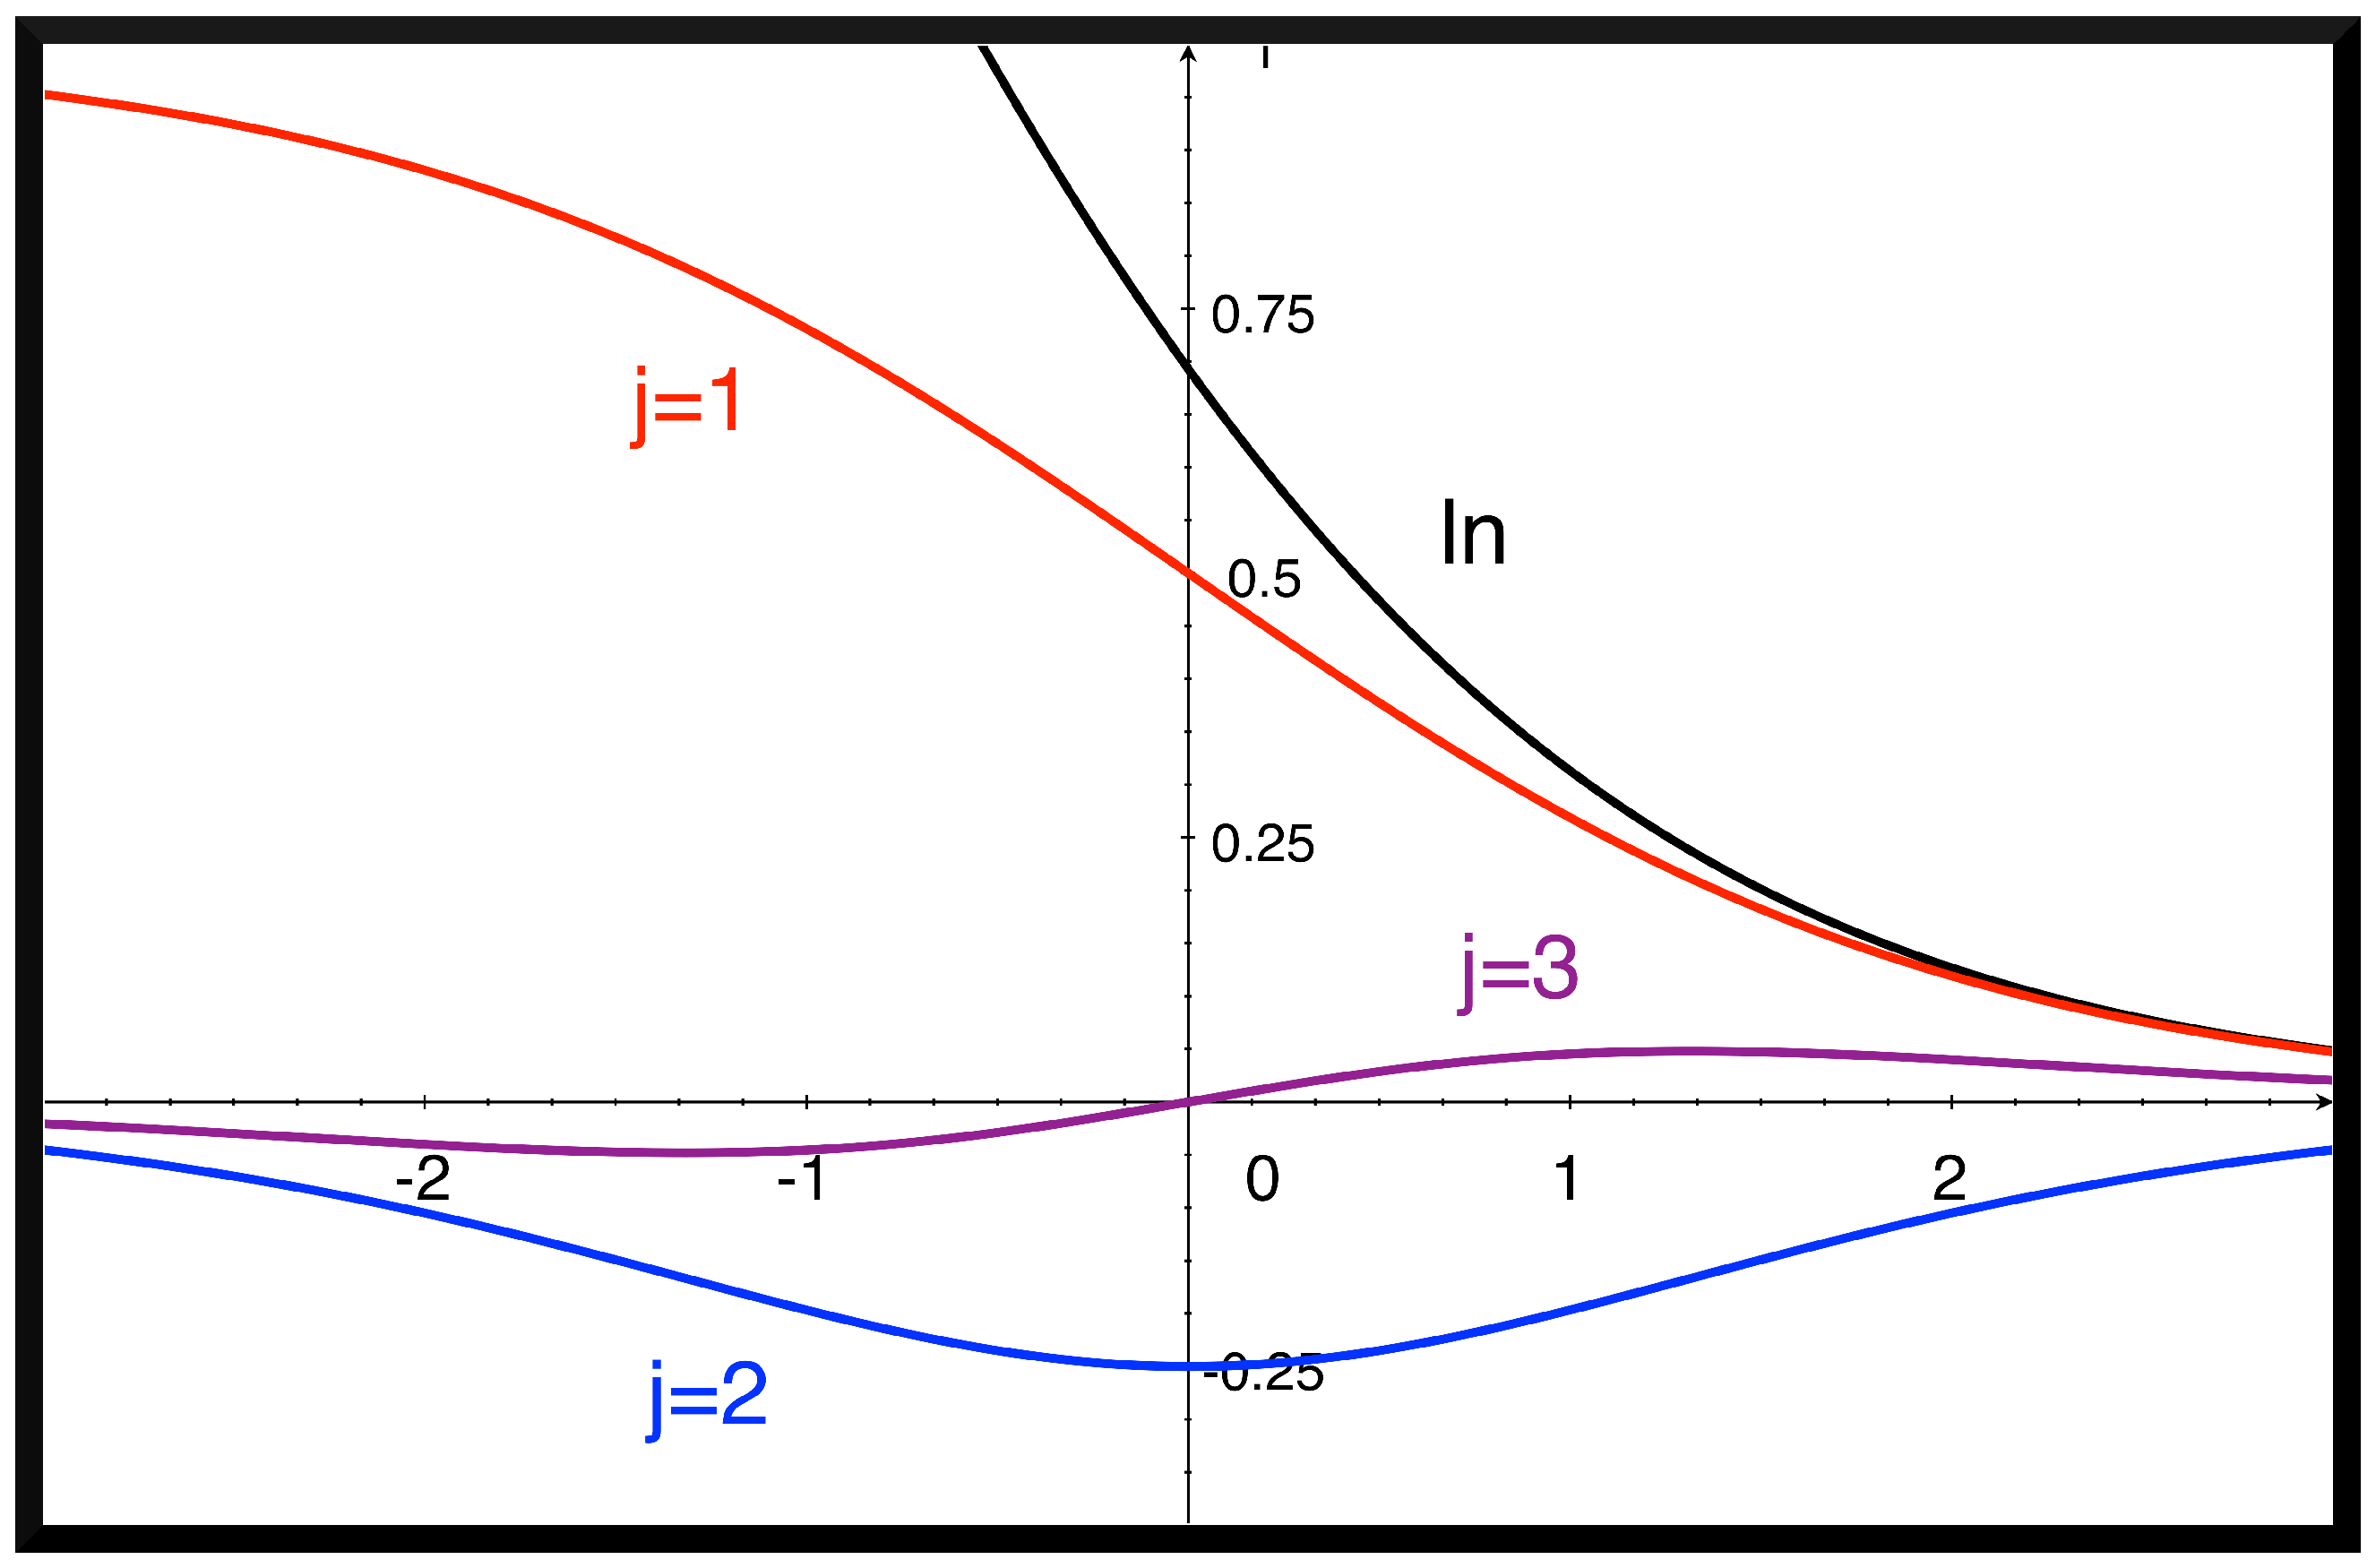
\includegraphics[width=0.5\linewidth,clip=true]
{Figs/Matsubarasums/matsubarasums1.eps}
\end{center}
\caption{\label{fig:matsubarasums} The result of Matsubara sums
  $-k_BT\sum_\nu\ln[-i\hbar\omega_\nu+\epsilon]$, $k_BT\sum_\nu
  \frac{1}{(i\hbar\omega_\nu-\epsilon)}\e{i\omega_\nu 0^+}$,
$k_BT\sum_\nu \frac{1}{(i\hbar\omega_\nu-\epsilon)^2}$ as
  function of energy $\epsilon$.}
\end{figure}

%==============================================================================
\subsubsection{Laurent expansion for the density matrix}
%==============================================================================
With this expression, we obtain the Matsubara sum required for the
density matrix as
\begin{eqnarray*}
\frac{1}{\beta}\sum_\nu\mat{G}\e{i\omega_\nu0^+}
&=&\sum_{j=1}^\infty
\left.\mat{\mathcal{G}}^{(j)}\frac{1}{(j-1)!}
\partial^{j-1}_\epsilon\right|_{\epsilon=0}(1+\e{\beta\epsilon})^{-1}
\nonumber\\
&=&
\frac{1}{2}\mat{\mathcal{G}}^{(1)}
-\frac{1}{4}\beta\mat{\mathcal{G}}^{(2)}
-0\cdot\beta^2\mat{\mathcal{G}}^{(3)}
+\underbrace{\Bigl(
\frac{1}{3!}\frac{1}{8}\beta^3\mat{\mathcal{G}}^{(4)}
-\frac{1}{5!}\frac{1}{4}\beta^5\mat{\mathcal{G}}^{(6)}
+\frac{1}{7!}1.0?\beta^7\mat{\mathcal{G}}^{(8)}\Bigr)
}_{\text{from grapher}}
+O(\beta^9)
\nonumber\\
&=&
\frac{1}{2}\mat{\mathcal{G}}^{(1)}
-\frac{1}{4}\beta\mat{\mathcal{G}}^{(2)}
+\underbrace{\Bigl(
\frac{1}{48}\beta^3\mat{\mathcal{G}}^{(4)}
-\frac{1}{480}\beta^5\mat{\mathcal{G}}^{(6)}
+\frac{1.0?}{4320}\beta^7\mat{\mathcal{G}}^{(8)}\Bigr)}_{\text{from grapher}}
+O(\beta^9)
\end{eqnarray*}

\clearpage
\bibliographystyle{unsrtnat}
\bibliography{../all}
\end{document}  
